\documentclass[11pt,a4paper]{article}
\usepackage{geometry}
\usepackage{amsmath}
\usepackage{amssymb}
\usepackage[utf8]{inputenc}  
\usepackage[T1]{fontenc}  
\usepackage{enumitem}
\usepackage{sectsty}
\usepackage{xcolor}
\usepackage{graphicx}
\usepackage{french}
\usepackage{float} 

% Marges
\geometry{hmargin=2.5cm,vmargin=2cm}

% On définit les deux couleurs utilisées
\definecolor{couleur_section}{RGB}{0,0,128}
\definecolor{couleur_subsection}{RGB}{0,128,255}

% On personnalise chacun des titres à l'aide des commandes "sectionfont", "subsectionfont", etc.
\sectionfont{\color{couleur_section} \scshape}
\subsectionfont{\color{couleur_subsection}}
\subsubsectionfont{\itshape}




\begin{document}

%% PAGE DE GARDE %%
\begin{titlepage}
	\centering
	
\includegraphics[width=0.40\textwidth]{uca.png}\par\vspace{1cm}
	{\scshape\LARGE Université Clermont Auvergne \par}
	{\scshape École Universitaire de Physique et d'Ingénierie \par}
	\vspace{2cm}
	\noindent\rule{\textwidth}{0.5pt}\par
	{\scshape\Large Etude d'un article scientifique de \textbf{Deep Learning}\par}
	\vspace{0.5cm}
	{\huge\bfseries Context Encoder\par}
	\noindent\rule{\textwidth}{0.5pt}\par
	\vspace{4cm}
	{\Large\itshape Lucas TOURON\par}
	{\Large\itshape Sagaf YOUSSOUF\par}

	\vfill

% Bottom of the page
	{\large 2019 - 2020\par}
\end{titlepage}

%% TABLE DES MATIERES %%
\tableofcontents
\newpage

%% CONTENU DU RAPPORT %%
\section{Matériel}
Dans cette section, je vais vous présenter tout le matériel que j'ai utilisé pour réaliser ce projet.


\subsection{Fe-Pi Audio Z V2}
Pour pouvoir acquérir et jouer le son de la guitare via le Raspberry Pi, j'ai décidé d'acquérir une carte son entrée/sortie : \textbf{Fe-Pi Audio Z V2}. Elle possède un codec NXP SGTL5000 \footnote{https://www.nxp.com/products/media-and-audio/audio-converters/audio-codec/ultra-low-power-audio-codec:SGTL5000} qui est orienté très basse consommation. Il dispose de : 
\begin{itemize}[noitemsep]
	\item deux entrées (micro ou stéréo) ;
	\item un bloc de traitement audio (réglage de tonalité, de basse...) ;
	\item un bus d'interface I2S pour communiquer avec le Raspberry Pi par exemple ;
	\item un PLL pour diviser la fréquence de l'horloge du système (ici celle de la Raspberry Pi) ;
	\item deux sorties (casque et stéréo).
\end{itemize}

\begin{figure}[H]
	\centering
	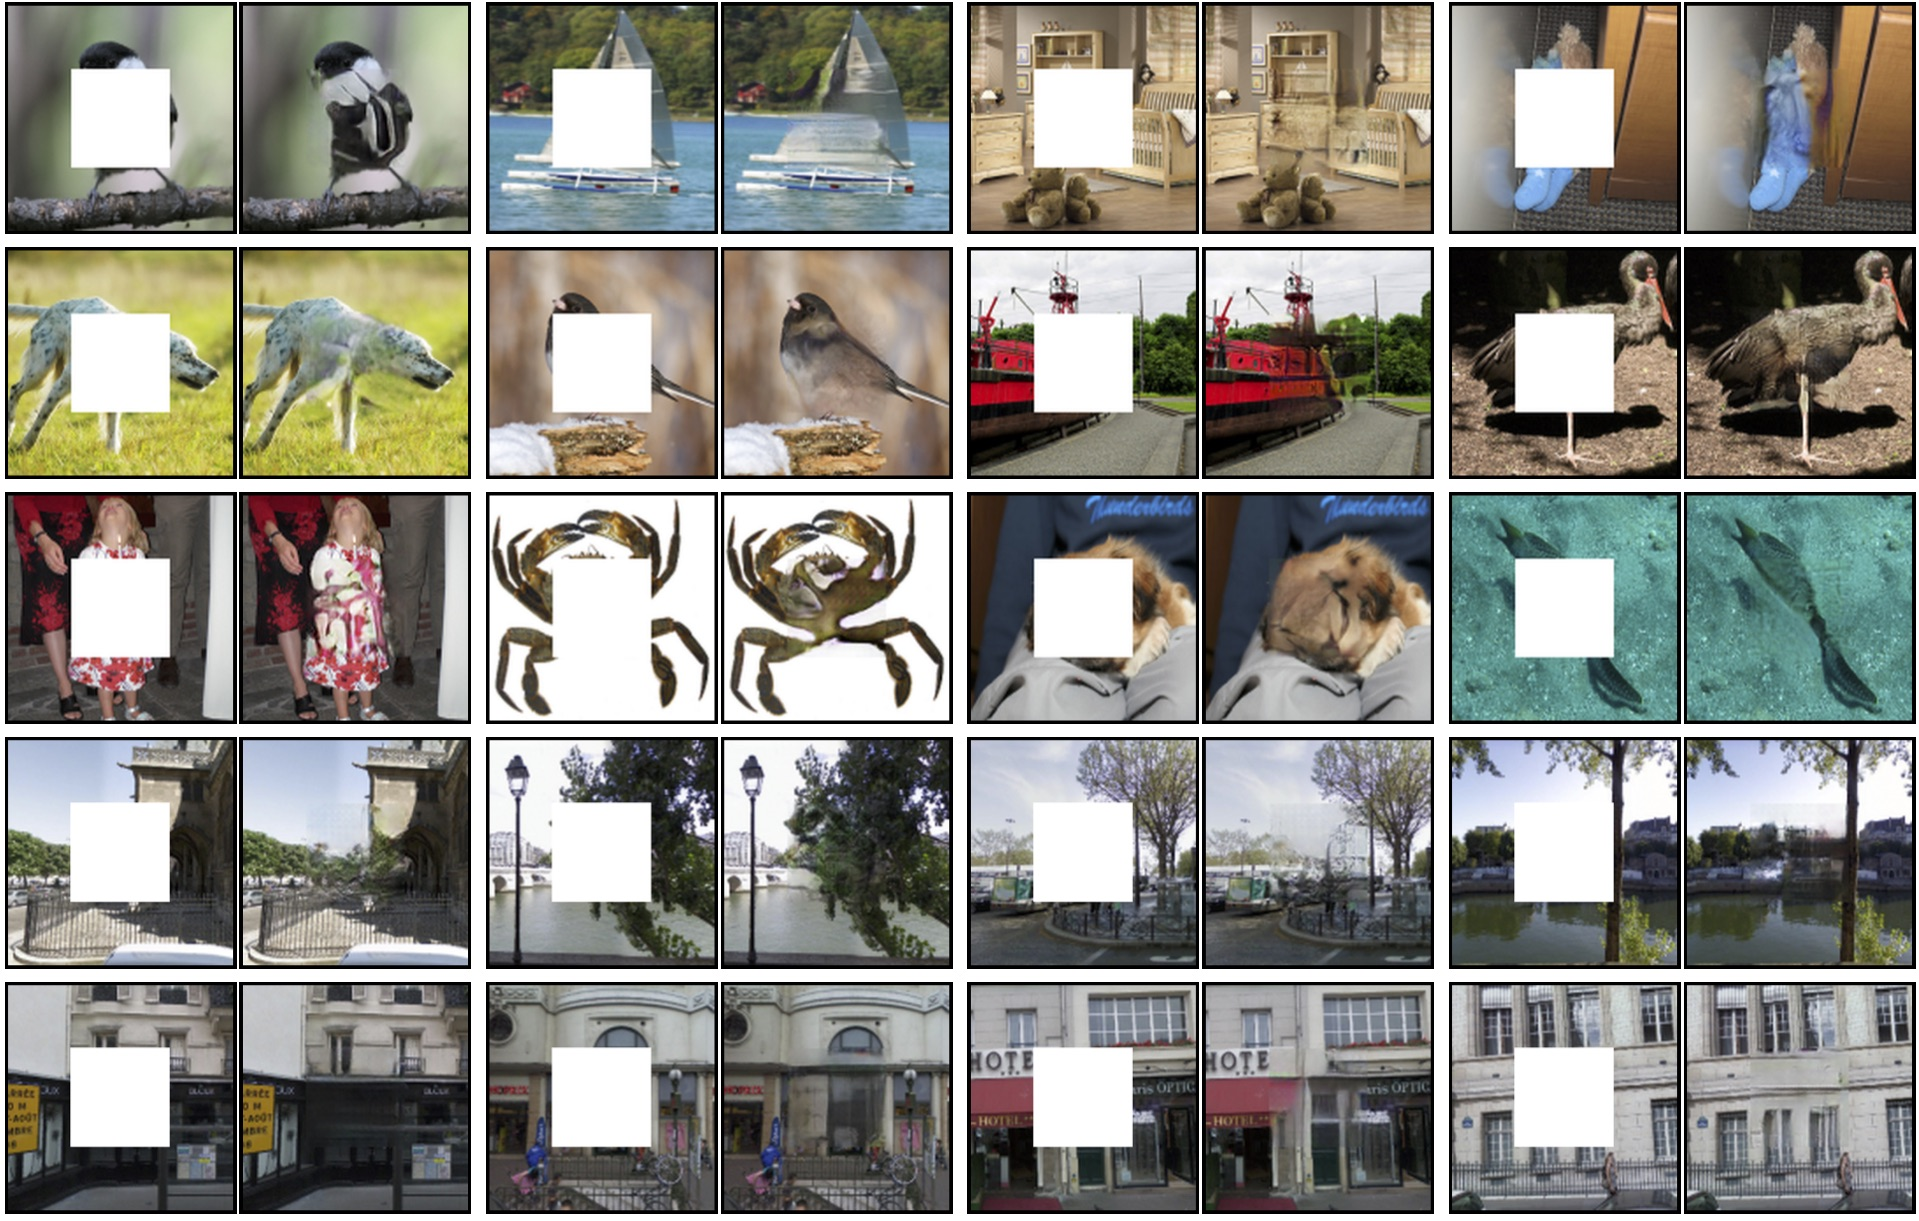
\includegraphics[scale=0.2]{teaser.jpg} 
	\caption{Exemples d'application}
\end{figure}




%% TABLE DES FIGURES %%
\newpage
\listoffigures
\newpage


\begin{thebibliography}{9}
\bibitem{latexcompanion} 
Michel Goossens, Frank Mittelbach, and Alexander Samarin. 
\textit{The \LaTeX\ Companion}. 
Addison-Wesley, Reading, Massachusetts, 1993.
 
\bibitem{einstein} 
Albert Einstein. 
\textit{Zur Elektrodynamik bewegter K{\"o}rper}. (German) 
[\textit{On the electrodynamics of moving bodies}]. 
Annalen der Physik, 322(10):891–921, 1905.
 
\bibitem{knuthwebsite} 
Knuth: Computers and Typesetting,
\\\texttt{http://www-cs-faculty.stanford.edu/\~{}uno/abcde.html}
\end{thebibliography}



\end{document}

